
\part*{Energie, Leistung und Potentiale}


\section*{Energie}


\subsection*{Mechanische Energie}

Wir definieren jetzt eine physikalische Grösse, die mechanische Energie:
\begin{verse}
$E_{mech}=\vec{F}\cdot\vec{s}=\left[Kraft\cdot Weg\right]=\left[J\right]=\left[\frac{kgm^{2}}{s^{2}}\right]$
\end{verse}

\subsection*{Potentielle Energie}
\begin{verse}
$E_{mech}=\vec{F}\cdot\vec{s}=\left[Kraft\cdot Weg\right]=\overset{h}{\underset{0}{\int}}F\cdot dh=\overset{h}{\underset{0}{\int}}mg\cdot dh=mgh$
\end{verse}
Um die Kugel zu heben, müssen Sie die mechanische Energie mgh investieren.
Die potentielle oder Lageenergie der Kugel wird dadurch um mgh erhöht.\\
Potentielle Energie im Gravitationsfeld = mgh
\begin{verse}
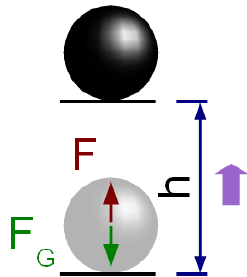
\includegraphics[scale=0.6]{Energie-Leistung-Potentiale/Potentielle_Energie}
\end{verse}

\subsection*{Kinetische Energie}
\begin{verse}
$E_{mech}=\vec{F}\cdot\vec{s}=Fs$

$F=ma$ (a = Beschleunigung)

$s=\frac{a}{2}t^{2}$ (Zusammenhang Strecke-Beschleunigung)

$v=at$

$\Rightarrow Fs=ma\cdot s=ma\cdot\frac{a}{2}t^{2}=m\cdot\frac{v^{2}}{2}$

$\Rightarrow E_{kin}=m\cdot\frac{v^{2}}{2}$
\end{verse}
Gilt allgemein, die gegebene Herleitung funktioniert allerdings nur
für konstante Kräfte.


\subsection*{Federenergie}
\begin{verse}
$\vec{F}_{s}=-k(x-L)\vec{e}_{x}$

$\vec{e}_{x}=$Einheitsvektor in x-Richtung

L = Ruhelänge

$E_{Feder}=\overset{x}{\underset{L}{\int}}Fdx=\overset{x}{\underset{L}{\int}}k(x-L)dx=\frac{k(x-L)^{2}}{2}$
\end{verse}
$\Rightarrow E_{kin}=m\cdot\frac{v^{2}}{2}$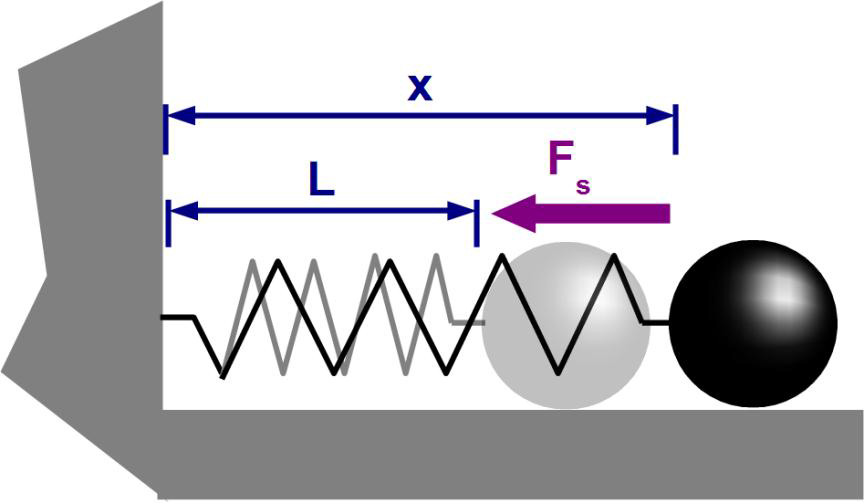
\includegraphics[scale=0.3]{Energie-Leistung-Potentiale/Federenergie}


\section*{Arbeit}
\begin{verse}
$\Delta W=\vec{F}\cdot\Delta\vec{r}$
\end{verse}
Dabei ist $\vec{F}$ eine Kraft und $\Delta\vec{r}$ ein Stück Weg.
Der Punkt bezeichnet das Skalarprodukt.


\subsection*{Skalarprodukt}
\begin{verse}
$\vec{a}\cdot\vec{b}=\left(\begin{array}{c}
a_{x}\\
a_{y}\\
a_{z}
\end{array}\right)\cdot\left(\begin{array}{c}
b_{x}\\
b_{y}\\
b_{z}
\end{array}\right)=a_{x}b_{x}+a_{y}b_{y}+a_{z}b_{z}$
\end{verse}
Geometrische Interpretation:
\begin{verse}
$\vec{a}\cdot\vec{b}=|\vec{a}|\cdot|\vec{b}|\cdot cos(\alpha)$

$\alpha=arccos(\frac{\vec{a}\cdot\vec{b}}{|\vec{a}|\cdot|\vec{b}|})=arccos(\frac{a_{x}b_{x}+a_{y}b_{y}+a_{z}b_{z}}{\sqrt{a_{x}^{2}+a_{y}^{2}+a_{z}^{2}}\cdot\sqrt{b_{x}^{2}+b_{y}^{2}+b_{z}^{2}}})$

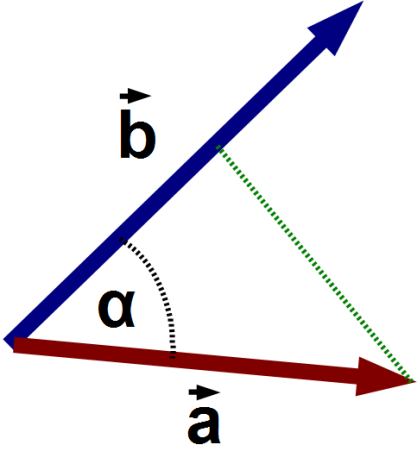
\includegraphics[scale=0.4]{Energie-Leistung-Potentiale/Skalarprodukt}

$|\vec{a}|=\sqrt{a_{x}^{2}+a_{y}^{2}+a_{z}^{2}}$
\end{verse}
Für das Produkt eines Verktors mit sich selber gilt:\\
(Zwischenwinkel ist null)
\begin{verse}
$\vec{a}\bullet\vec{a}=|\vec{a}|\cdot|\vec{a}|\cdot cos(0)=|\vec{a}|^{2}$

$\Rightarrow E_{kin}=m\cdot\frac{\vec{v}^{2}}{2}=m\cdot\frac{\vec{v}\cdot\vec{v}}{2}=m\cdot\frac{|\vec{v}|^{2}}{2}$
\end{verse}

\section*{Energieerhaltung}


\subsection*{Energieerhaltungssatz}

Die Gesamtmenge der Energie in einem Prozess bleibt immer exakt erhalten.


\subsection*{Anwendung der Energieerhaltung}

Ansatz: Wenn die Kugel fällt, sinkt ihre potentielle Energie. Wegen
der Energieerhaltung steigt die kinetische Energie um einen entsprechenden
Betrag.
\begin{verse}
$E_{pot}(t)=mgh(t)$

$E_{kin}(t)=m\frac{v^{2}(t)}{2}$

$E_{pot}(t)+E_{kin}(t)=const.$

$E_{pot}(0)+E_{kin}(0)=mgH+0=mgH$

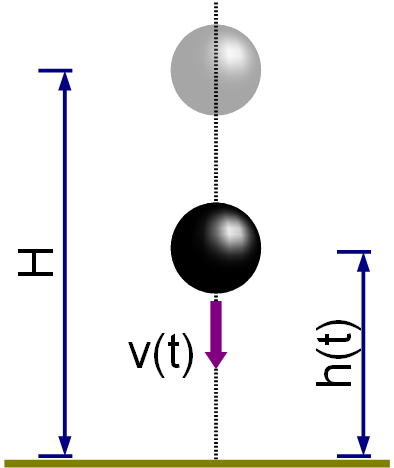
\includegraphics[scale=0.5]{Energie-Leistung-Potentiale/Energieerhaltung}

$mgH=mgh(t)+m\frac{v^{2}(t)}{2}$

$\Rightarrow v(t)=\sqrt{2g(H-h(t))}$
\end{verse}

\subsection*{Energie- und Impulserhaltung}


\subsubsection*{Impulserhaltung}
\begin{verse}
$m_{1}u_{1}+m_{2}u_{2}=m_{1}v_{1}+m_{2}v_{2}=P$
\end{verse}

\subsubsection*{Energierhaltung}
\begin{verse}
$m_{1}\frac{u_{1}^{2}}{2}+m_{2}\frac{u_{2}^{2}}{2}=m_{1}\frac{v_{1}^{2}}{2}+m_{2}\frac{v_{2}^{2}}{2}=E$

$v_{1}=\frac{(m_{1}-m_{2})\cdot u_{1}+2m_{2}u_{2}}{m_{1}+m_{2}}$

$v_{2}=\frac{(m_{2}-m_{1})\cdot u_{2}+2m_{1}u_{1}}{m_{1}+m_{2}}$
\end{verse}
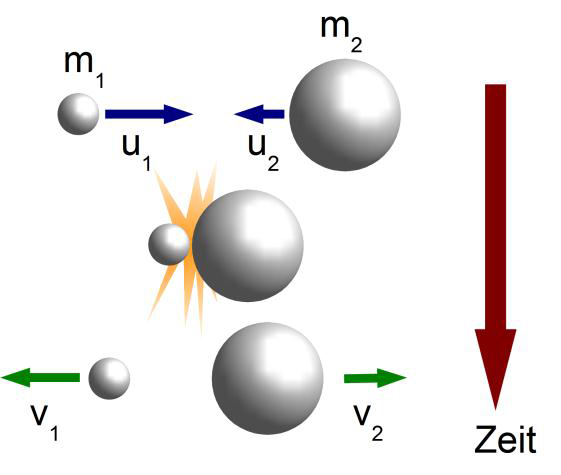
\includegraphics[scale=0.5]{Energie-Leistung-Potentiale/Impulserhaltung}


\section*{Potentiale}


\subsection*{Dissipative und Konservative Systeme}
\begin{itemize}
\item Ein System heisst konservativ, wenn die Summe der Energien seiner
Komponenten erhalten bleibt.
\item Ein System heisst dissipativ, wenn es Energie in die Umwelt abgibt
(z.B. durch Wärmestrahlung oder Reibung)
\end{itemize}

\subsection*{Potentielle Energie}

Definition: Differenz der potentiellen Energien zwischen zwei Punkten
= Arbeit, die es braucht, eine Masse vom ersten zum zweiten Punkt
zu bringen.\\
Falls wir die potentielle Energie eines Objekts als Funktion der Lage
angeben können (und nicht weiter sagen müssen, wie wir vom Anfangs-
zum Endpunkt eines Pfads gelangen), haben wir es mit einem Potential
zu tun.


\section*{Leistung}
\begin{itemize}
\item Leistung ist Energie pro Zeit = $\left[W\right]=\left[\frac{J}{s}\right]$
\item $1kwH=3.6\cdot10^{6}Ws=3.6\cdot10^{6}J$
\end{itemize}

\subsection*{Bilanzmodelle}

Ausgleich zwischen Energiespeichern findet über Ströme von „Energieträgern“
statt:
\begin{verse}
$Strom=\frac{Energietr\ddot{a}ger}{Zeit}$
\end{verse}
Damit Sie mit einem Energieträgerstrom eine Leistung berechnen können,
müssen Sie wissen, wieviel Energie in einem Energieträger steckt:
\begin{verse}
$\frac{Energie}{Zeit}=\frac{Energie}{Energietr\ddot{a}ger}\cdot\frac{Energietr\ddot{a}ger}{Zeit}=Potentialdifferenz\cdot Strom$
\end{verse}

\subsection*{Stoffe, Potential, Energie}

\begin{tabular}{|c|c|c|c|c|}
\hline 
Gebiet & Stoffmenge & Potential & Energie & Leistung\tabularnewline
\hline 
\hline 
Elektrizität & Ladung Q & Spannung U & $E=U\cdot Q$ & $P=U\cdot I_{q}$\tabularnewline
\hline 
Hydraulik & Volumen V & Druck p & $E=p\cdot V$ & $P=\Delta p\cdot I_{v}$\tabularnewline
\hline 
Gravitation & Masse m & $E=g\cdot h$ & $E=m\cdot g\cdot h$ & $P=g\cdot\Delta h\cdot I_{m}$\tabularnewline
\hline 
\end{tabular}
